\documentclass[border=10pt]{standalone}
\usepackage[svgnames]{xcolor}
\usepackage{amsmath}
\usepackage{pgfplots}
\pgfplotsset{compat=newest}
\usepackage[sfdefault]{FiraSans}
\usepackage{FiraMono}
\renewcommand*\familydefault{\sfdefault}
\begin{document}
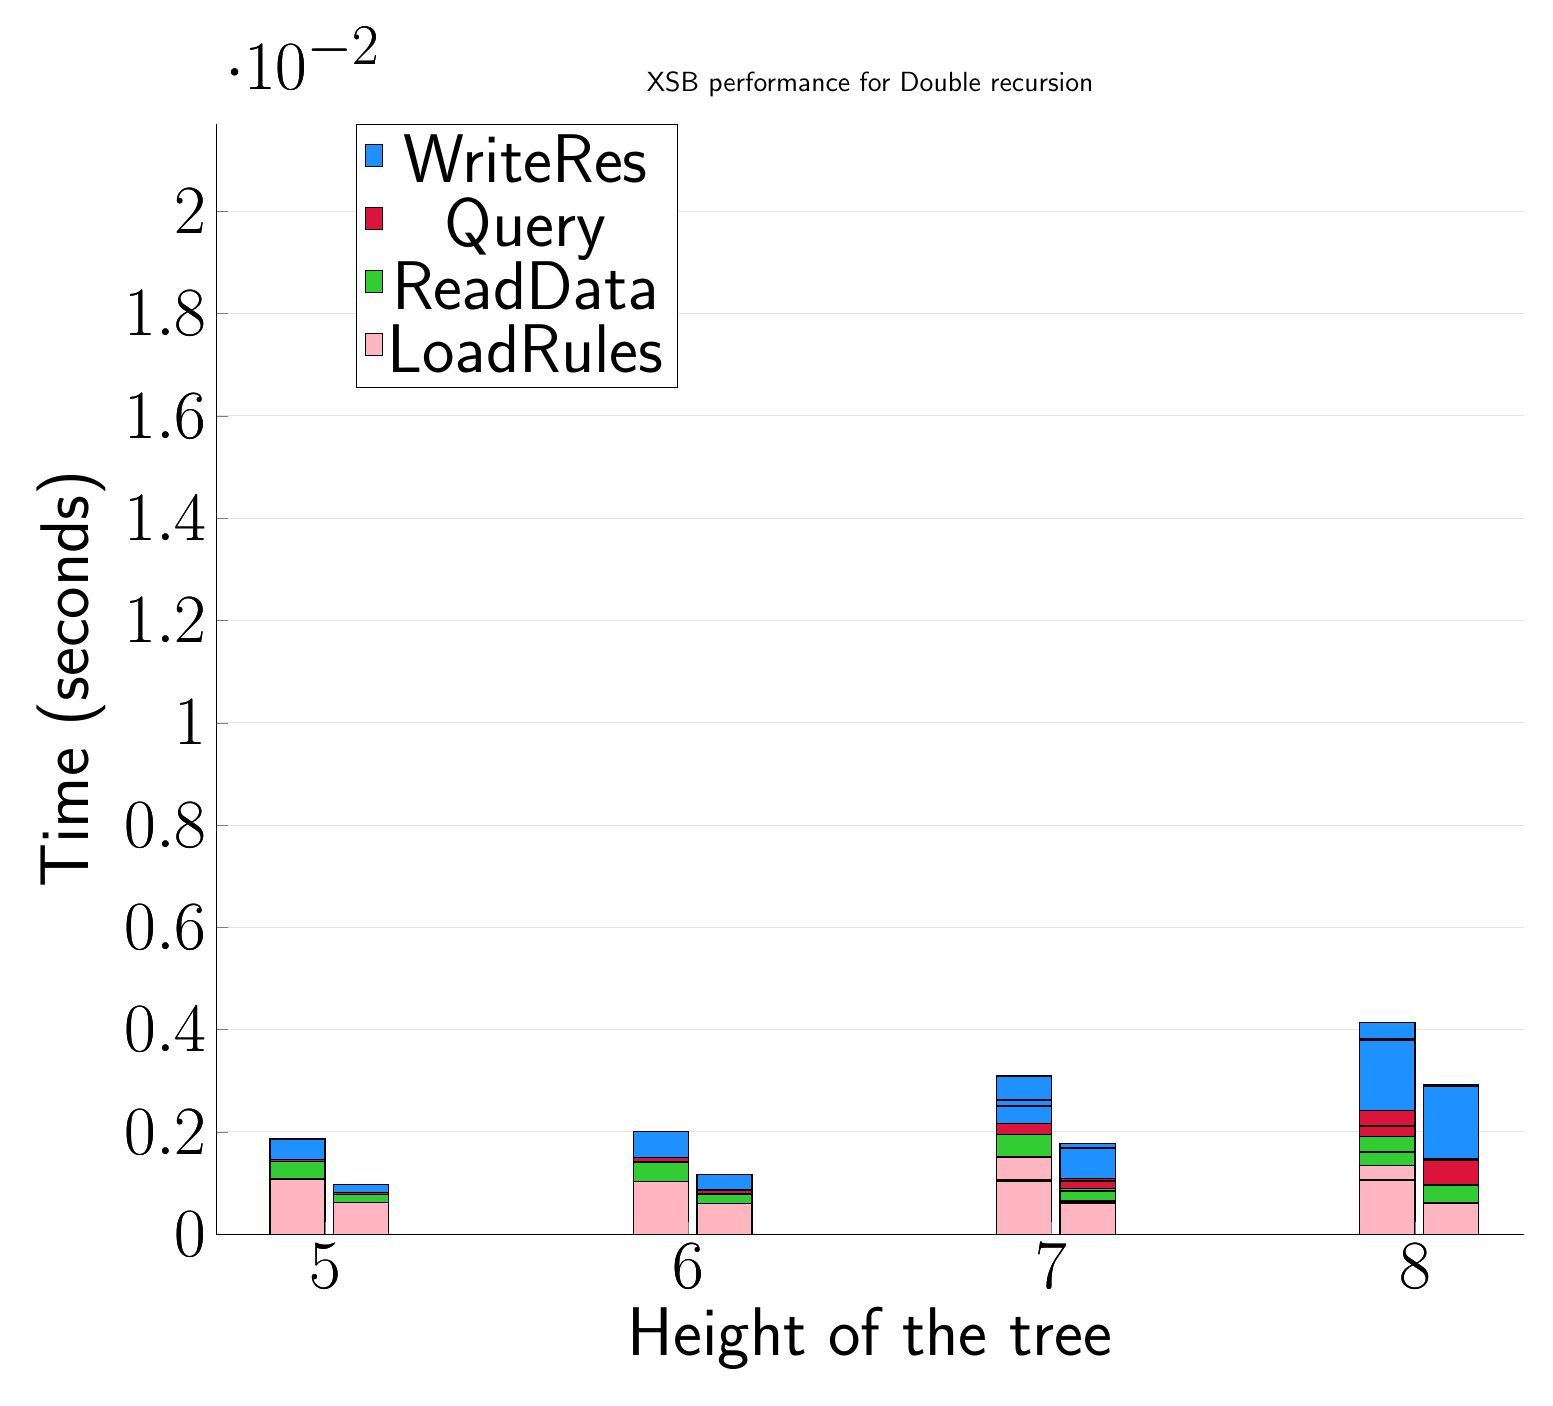
\begin{tikzpicture}
\begin{axis}[
   ybar stacked,
   title={XSB performance for Double recursion},
   bar shift=-10pt,
   width=1.5\textwidth,
   bar width=0.7cm,
   ymajorgrids, tick align=inside,
   major grid style={draw=gray!20},
   xtick=data,
   ymin=0, ymax=0.021717853546142578,
   axis x line*=bottom,
   axis y line*=left,
   enlarge x limits=0.1,
   legend style={
       at={(0.23, 1)},
       anchor=north,
       legend columns=1,
       font=\Huge,
   },
   ylabel={Time (seconds)},
   xlabel={Height of the tree},
   label style={font=\Huge},
   tick label style={font=\Huge},
]
\addlegendimage{fill=DodgerBlue, draw=black, line width=0.2pt}
\addlegendentry{WriteRes}
\addlegendimage{fill=Crimson, draw=black, line width=0.2pt}
\addlegendentry{Query}
\addlegendimage{fill=LimeGreen, draw=black, line width=0.2pt}
\addlegendentry{ReadData}
\addlegendimage{fill=LightPink, draw=black, line width=0.2pt}
\addlegendentry{LoadRules}
\addplot +[fill=LightPink, draw=black, line width=0.5pt] coordinates {
    (5, 0.001076221466064453)
    (6, 0.001036143302917479)
    (7, 0.001075935363769531)
    (7, 0.001501250267028808)
    (7, 0.0010370731353759781)
    (8, 0.001047611236572267)
    (8, 0.0010571956634521477)
    (8, 0.001339316368103027)
};
\addplot +[fill=LimeGreen, draw=black, line width=0.5pt] coordinates {
    (5, 0.0003440380096435548)
    (6, 0.00037612915039062503)
    (7, 0.00044236183166503925)
    (7, 0.00045056343078613264)
    (7, 0.0004172086715698244)
    (8, 0.0005656242370605469)
    (8, 0.0005515575408935548)
    (8, 0.0005665063858032226)
};
\addplot +[fill=Crimson, draw=black, line width=0.5pt] coordinates {
    (5, 4.4012069702148456e-05)
    (6, 8.478164672851563e-05)
    (7, 0.0002021074295043945)
    (7, 0.0002118110656738282)
    (7, 0.0001998186111450194)
    (8, 0.0005077600479125976)
    (8, 0.0005064010620117188)
    (8, 0.0005112409591674805)
};
\addplot +[fill=DodgerBlue, draw=black, line width=0.5pt] coordinates {
    (5, 0.0003960132598876953)
    (6, 0.00050811767578125)
    (7, 0.0009009361267089845)
    (7, 0.0009284734725952147)
    (7, 0.0008541822433471697)
    (8, 0.0016962051391601566)
    (8, 0.001685857772827149)
    (8, 0.0017178535461425774)
};
\end{axis}
\begin{axis}[
   ybar stacked,
   bar shift=13pt,
   width=1.5\textwidth,
   bar width=0.7cm,
   ymajorgrids, tick align=inside,
   major grid style={draw=none},
   xtick=data,
   ymin=0, ymax=0.021717853546142578,
   axis x line*=none,
   axis y line*=none,
   enlarge x limits=0.1,
   label style={font=\Huge},
   tick label style={font=\Huge},
]
\addplot +[fill=LightPink, draw=black, line width=0.5pt] coordinates {
    (5, 0.0006166)
    (6, 0.0006020999999999997)
    (7, 0.0006108999999999995)
    (7, 0.0006471999999999997)
    (7, 0.0005997)
    (8, 0.0006013000000000001)
    (8, 0.0006070000000000002)
    (8, 0.0006232999999999996)
};
\addplot +[fill=LimeGreen, draw=black, line width=0.5pt] coordinates {
    (5, 0.0001583999999999999)
    (6, 0.00018540000000000036)
    (7, 0.00024080000000000027)
    (7, 0.0002461000000000004)
    (7, 0.0002336000000000001)
    (8, 0.0003510999999999999)
    (8, 0.0003472000000000003)
    (8, 0.00035470000000000044)
};
\addplot +[fill=Crimson, draw=black, line width=0.5pt] coordinates {
    (5, 3.770000000000024e-05)
    (6, 7.889999999999979e-05)
    (7, 0.0001936999999999998)
    (7, 0.00020159999999999997)
    (7, 0.00019170000000000021)
    (8, 0.0004874999999999999)
    (8, 0.00048780000000000004)
    (8, 0.0004896999999999994)
};
\addplot +[fill=DodgerBlue, draw=black, line width=0.5pt] coordinates {
    (5, 0.00016019999999999996)
    (6, 0.0003022000000000003)
    (7, 0.0006552000000000001)
    (7, 0.0006832000000000003)
    (7, 0.0006492999999999998)
    (8, 0.0014538000000000003)
    (8, 0.0014422999999999999)
    (8, 0.0014503000000000007)
};
\end{axis}
\end{tikzpicture}

\end{document}
